\documentclass[aspectratio=169,t]{beamer}

% Clean academic look: white background, no decorations, generous whitespace.
\usetheme{default}
\setbeamertemplate{navigation symbols}{}
\setbeamercolor{background canvas}{bg=white}
\setbeamercolor{normal text}{fg=black!88}
\setbeamercolor{frametitle}{fg=black}
\setbeamerfont{frametitle}{size=\Large, series=\bfseries}
\setbeamertemplate{frametitle}{%
  \vspace{0.7em}\hspace{0.5em}\insertframetitle\par%
  \vspace{0.2em}\hspace{0.6em}{\small\color{black!55}\insertframesubtitle}\par}
\setbeamertemplate{footline}{%
  \hfill\scriptsize\color{black!35}\insertframenumber\;/\;\inserttotalframenumber\hspace{1em}\vspace{0.5em}}
\setbeamertemplate{itemize item}{\textbullet}
\setbeamertemplate{itemize subitem}{\textendash}

\usepackage{booktabs}
\usepackage{amsmath, amssymb}
\usepackage{xcolor}
\usepackage{graphicx}
\usepackage{tabularx}
\usepackage{array}
\usepackage{tikz}
\usetikzlibrary{matrix, positioning, arrows.meta}

% Compact tables, gentle row spacing
\renewcommand{\arraystretch}{1.10}

% Where ggsave outputs live (relative to the .tex compile dir)
\graphicspath{{./}{../figs/}{../figs/longitudinal/}{../figs/io/}{../figs/proc/}{../figs/schematic/}}

% Convenience commands
\newcommand{\pia}{\pi_{\alpha}}
\newcommand{\sigxi}{\sigma_{\xi}}
\newcommand{\siga}{\sigma_{\alpha}}
\newcommand{\sigr}{\sigma_{r}}
\newcommand{\sigz}{\sigma_{\zeta}}
\newcommand{\siglam}{\sigma_{\lambda}}
\newcommand{\sigs}{\sigma_{s}}
\newcommand{\kappap}{\kappa_{\text{pop}}}

% Recurring outline slide at each section start. Shows the full TOC with
% the current section highlighted.
\AtBeginSection[]{%
  \begin{frame}{Outline}
    \vspace{0.5em}
    \tableofcontents[currentsection,
                     sectionstyle=show/shaded,
                     subsectionstyle=hide]
  \end{frame}
}
\setbeamertemplate{section in toc}{%
  \leavevmode\leftskip=1em%
  \inserttocsectionnumber.\,\inserttocsection\par%
}

% Accent: brand-red used for the "kid" / acceleration thread
\definecolor{accent}{RGB}{195,30,55}
\definecolor{cool}{RGB}{31,120,180}

\title{\bfseries Acceleration and variability in the\\growth of children's early vocabulary}
\subtitle{}
\author{Michael C.\ Frank}
\institute{\small Stanford University}
\date{2026}

\begin{document}

% =====================================================================
\begin{frame}[plain]
\titlepage
\end{frame}

% =====================================================================
\begin{frame}{Vocabulary growth: rapid, variable, consequential}

\begin{columns}[T, onlytextwidth]
\column{0.55\textwidth}
\textbf{Theoretical:} Growth mechanisms are diagnostic of how
children's learning works --- and how it changes with development.

\vspace{1em}
\textbf{Practical:} Variation in vocabulary growth is a key precursor
of academic outcomes.

\vspace{1em}
\textbf{Methodological:} Vocabulary count has a property nearly no
other psychological metric has --- a \emph{true zero}. Children at
birth know zero words. Absolute variability in word counts is
interpretable, not just z-scores.

\column{0.45\textwidth}
\centering
\includegraphics[width=\linewidth]{precursor_acceleration.png}

\vspace{0.3em}
\scriptsize\color{black!55}\textit{Wordbank English (American) vocabulary
vs.\ age, with quantile fan: rapid growth, large between-child spread,
both diagnostic of learning.}
\end{columns}

\end{frame}

% =====================================================================
\begin{frame}{The data: Wordbank CDI}{What we measure when we measure a child's vocabulary}

\begin{columns}[T, onlytextwidth]
\column{0.55\textwidth}
\small
The MacArthur--Bates Communicative Development Inventory (CDI) is a
parent-report checklist of ~680 words. Parents indicate which words
their child \emph{produces} (Words \& Sentences) or
\emph{comprehends} (Words \& Gestures).

\vspace{0.7em}
\textbf{Wordbank}: open repository of CDI administrations across
~30 languages, ~$10^5$ children. Data we use here:
\begin{itemize}\setlength\itemsep{0.1em}
\item \textbf{Cross-sectional}: each child contributes one snapshot
\item \textbf{Longitudinal}: each child contributes $\geq$2 admins,
      letting us track per-child growth
\end{itemize}

\vspace{0.7em}
\textbf{Strong properties:} large $N$, parent-report calibrated against
direct testing, cross-linguistically validated, free-to-use.

\column{0.45\textwidth}
\centering
\includegraphics[width=\linewidth]{precursor_acceleration.png}

\vspace{0.3em}
\scriptsize\color{black!55}\textit{One child = one point.
A standard view of vocabulary $\times$ age in Wordbank English (American)
WS, with quantile-regression overlays at the 10/25/50/75/90th percentiles.}
\end{columns}

\end{frame}

% =====================================================================
\begin{frame}{The two signatures of vocabulary growth}{Both visible in any reasonably-sized vocabulary sample}

\centering
\includegraphics[width=0.78\linewidth]{precursor_acceleration.png}

\vspace{0.5em}
\small
\begin{columns}[T, onlytextwidth]
\column{0.5\textwidth}
\textbf{Signature 1: acceleration.}
Each quantile curve is concave up: doubling age more than doubles
vocabulary. The growth rate accelerates.
\column{0.5\textwidth}
\textbf{Signature 2: variability.}
The quantile lines fan out: between-child differences in vocabulary
grow with age, not shrink.
\end{columns}

\vspace{0.8em}
\small\textbf{These signatures are remarkably robust:} replicate across
languages, samples, and forms. Any model of early word learning must
explain both.

\end{frame}

% =====================================================================
\begin{frame}{The dominant theoretical view: pure accumulation}{Vocabulary as a counter that fills}

\begin{columns}[T, onlytextwidth]
\column{0.55\textwidth}
\small
The pure accumulator: each child has an input rate $r_i$ (words per hour);
each word $j$ has a difficulty $\delta_j$. A word is acquired when
enough tokens of it have accumulated.

\vspace{0.6em}
A textbook lineage:
\begin{itemize}\setlength\itemsep{0.15em}
\item \textbf{McMurray (2007).}\, Pure rate-times-time accumulator.
\item \textbf{Mitchell \& McMurray (2009).}\, + leverage feedback.
\item \textbf{Hidaka (2013).}\, Cumulative-Weibull; allows rate change.
\item \textbf{Mollica \& Piantadosi (2017).}\, Per-word Gamma waiting.
\item \textbf{Kachergis et al.\ (2021).}\, IRT Rasch with $\alpha_i$.
\end{itemize}

\vspace{0.5em}
\textbf{All share}: between-child variation is in baseline ($r_i$ or
$\alpha_i$); per-child scaling exponent is implicitly fixed.

\column{0.45\textwidth}
\centering
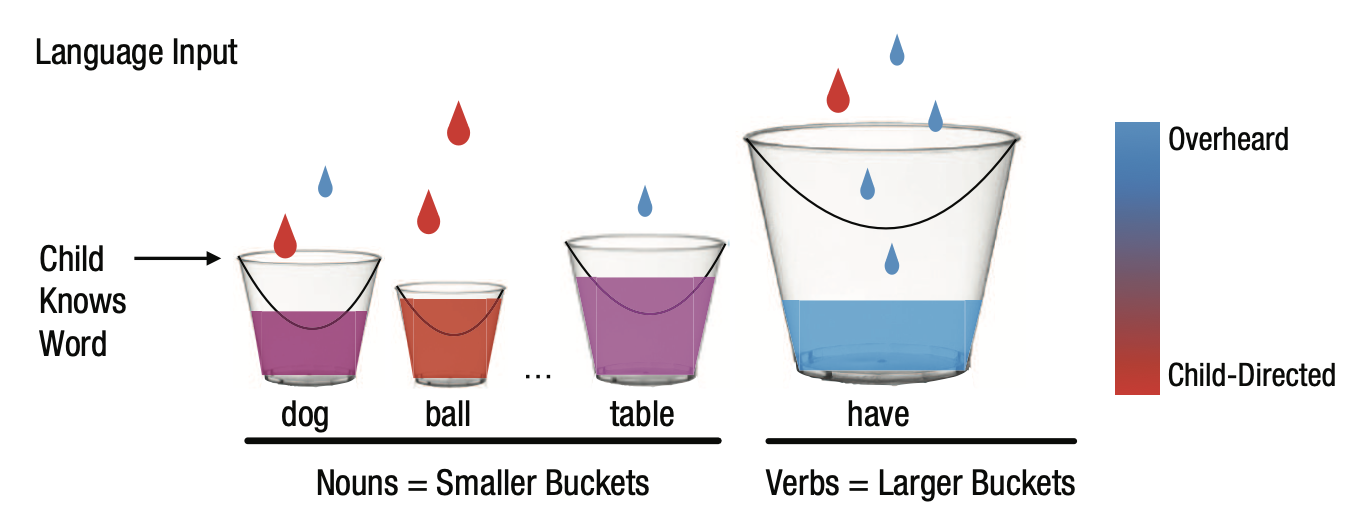
\includegraphics[width=0.95\linewidth]{kachergis_buckets.png}

\vspace{0.3em}
\scriptsize\color{black!55}\textit{Bucket-fill metaphor: each child
hears tokens at rate $r_i \cdot p_j$; word $j$ is acquired when its
bucket fills past difficulty $\delta_j$.}
\end{columns}

\end{frame}

% =====================================================================
\begin{frame}{The empirical gap: input matters less than supposed}{Coffey \& Snedeker (2026): meta-analytic $R^2$ = 0.04--0.07}

\begin{columns}[T, onlytextwidth]
\column{0.55\textwidth}
\small
The accumulator view predicts that variation in vocabulary growth is
dominated by variation in input quantity. But Coffey \& Snedeker (2026)
meta-analyzed 71 input studies, 4,760 children:

\vspace{0.5em}
\textbf{Input $\to$ outcome $R^2$ across four input measures: 0.04--0.07.}

\vspace{0.7em}
That is: \emph{caregiver speech quantity explains 4--7\% of variance
in language outcome}. The relationship is real but small.

\vspace{0.5em}
The dominant accumulator view leaves a \textbf{huge variance budget}
unexplained --- where does the other 90+\% live?

\vspace{0.7em}
\textbf{Our hypothesis}: in \emph{how children accelerate}, not just
how much input they hear. Modeling this requires freeing two
parameters that prior models pin: per-child acceleration and per-child
trajectory phase.

\column{0.45\textwidth}
\centering
\includegraphics[width=0.95\linewidth]{precursor_variability.png}

\vspace{0.3em}
\scriptsize\color{black!55}\textit{Between-child variability in
ability $\theta$ (1-PL Rasch IRT) grows from $\sim$1.7 logits at 16 mo
to $\sim$2.3 logits at 30 mo. If input quantity explains only $\sim$5\%
of this, the rest must come from elsewhere.}
\end{columns}

\end{frame}

% =====================================================================
\begin{frame}{This work: modeling individual variability in acceleration}

\small
We build a Bayesian IRT-accumulator model that pins down three
quantities directly:

\vspace{0.6em}
\begin{itemize}\setlength\itemsep{0.5em}
\item \textbf{The acceleration signature.} Is population vocabulary
  growth super-linear in cumulative input? ($\kappap > 1$?)
\item \textbf{The variability signature.} Do children differ in their
  scaling exponent and trajectory phase, not just baseline?
  ($\sigz > 0$? $\sigs > 0$?)
\item \textbf{The input share.} How much of between-child variance is
  attributable to input rate vs.\ to internal factors?
  ($\pia = \siga^2 / (\siga^2 + \sigr^2)$.)
\end{itemize}

\vspace{0.8em}
We then ask: does the same machinery applied to large language models
yield the same answers? \textbf{Spoiler}: no --- LLMs show a categorical
disanalogy with children's learning. (Later in the talk.)

\end{frame}

% =====================================================================
\section{Two empirical signatures: acceleration and variability}

% =====================================================================
\begin{frame}{Acceleration: vocabulary grows super-linearly with age}

\centering
\includegraphics[width=0.78\linewidth]{precursor_acceleration.png}

\vspace{0.4em}
\small
\textbf{Each line is a percentile (10/25/50/75/90) of vocabulary across kids.}
The concave-up shape across the productive window (16--30 mo) is the
visual signature of super-linear growth: doubling age does \emph{more}
than double vocabulary.

\end{frame}

% =====================================================================
\begin{frame}{Variability: between-child spread grows with age}

\centering
\includegraphics[width=0.78\linewidth]{precursor_variability.png}

\vspace{0.4em}
\small
\textbf{Children fan out, not converge.} Within-age SD of latent ability
$\theta$ (1-PL Rasch IRT) climbs from $\sim$1.7 logits at 16 mo to
$\sim$2.3 logits at 30 mo --- the spread grows even as kids age.

\end{frame}

% =====================================================================
\begin{frame}{Cross-language replication}{Variability and growth-with-age across Wordbank languages}

\centering
\includegraphics[width=0.78\linewidth]{precursor_crosslang_overlay.png}

\vspace{0.4em}
\small
\textbf{Variability is universal} --- and grows with age in every sampled language.
Each grey line is one language's within-age SD of $\theta_{\text{admin}}$;
red is the cross-language mean.

\end{frame}

% =====================================================================
\section{Building the model: individual variability in acceleration}

% =====================================================================
\begin{frame}{The structural null: pure accumulator}

\begin{columns}[T, onlytextwidth]
\column{0.55\textwidth}
\small
\textbf{Pure accumulator.}
Each child accumulates word-evidence at per-child input rate $r_i$;
word $j$ is acquired when difficulty $\delta_j$ is crossed.

\vspace{0.4em}
\textbf{Scaling exponent $\kappa_i$:} ability scales as (tokens)$^{\kappa_i}$.

\begin{itemize}\setlength\itemsep{0.15em}
\item $\kappa_i = 1$ for every child: pure unit accumulator.
\item Between-child variance comes only from $\sigma_r$ (input rate).
\item No per-child slope variation.
\end{itemize}

\vspace{0.4em}
\textbf{Two estimands diagnose deviation:}
$\boldsymbol{\sigma_\alpha}$ (efficiency variation) and the $\boldsymbol{\kappa_i}$
posterior (\emph{is $\kappa$ above 1, and does it vary?}).

\column{0.45\textwidth}
\centering
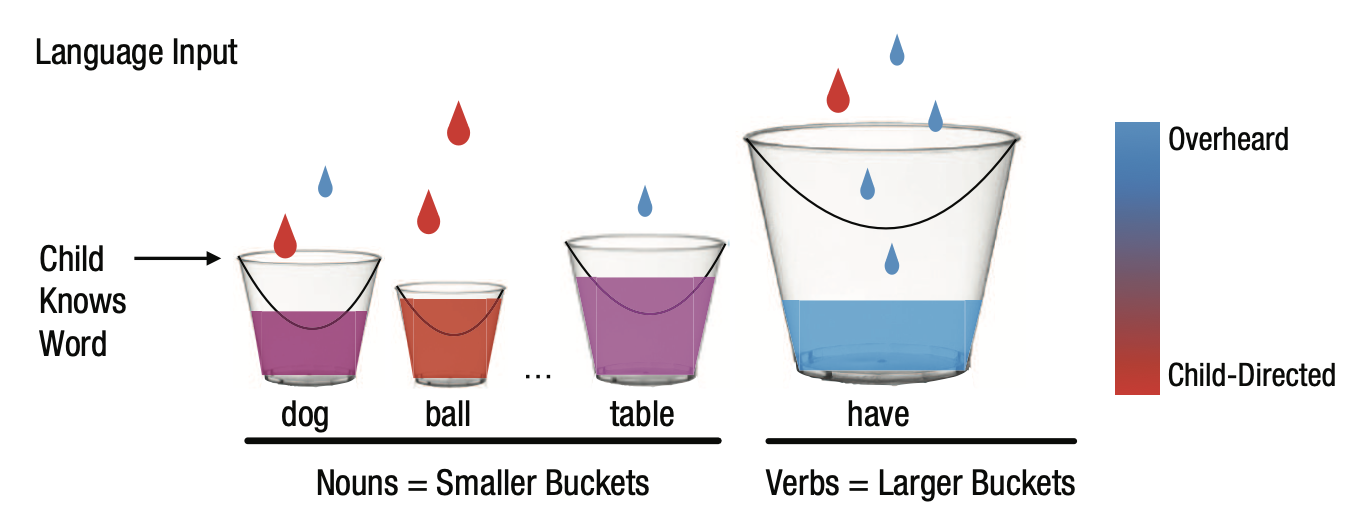
\includegraphics[width=0.92\linewidth]{kachergis_buckets.png}

\vspace{0.3em}
\scriptsize\color{black!55}\textit{Bucket-fill metaphor: each child
hears tokens at rate $r_i \cdot p_j$; word $j$ is acquired when its
bucket fills past difficulty $\delta_j$ (Kachergis et al.\ 2021).}
\end{columns}

\end{frame}

% =====================================================================
\begin{frame}{Prior accumulator models: structural lineage}{We'll translate each into our notation later, after the model build}

\small
\begin{description}\setlength\itemsep{0.5em}
\item[McMurray (2007).]
  Pure accumulator. Each word $w$ has acquisition threshold $\tau_w$
  from population distribution $g(\tau)$. Acceleration requires $g'(\tau) > 0$.
\item[Mitchell \& McMurray (2009).]
  McMurray $+$ leverage feedback $a(t) = t + cL(t)$. \emph{Shifts}
  growth without creating acceleration.
\item[Hidaka (2013).]
  Closed-form AoA distributions: cumulative (Gamma), rate-change
  (Weibull, exponent $D$ on time), or both.
\item[Mollica \& Piantadosi (2017).]
  Per-word Gamma waiting time: AoA $\sim \Gamma(k_w, \lambda_w)$.
\item[Kachergis et al.\ (2021).]
  1-PL Rasch IRT with per-child $\theta_i$ and linear age covariate.
\end{description}

\vspace{0.5em}
\small\color{black!55}\textit{Each uses different notation. After we
introduce our model, we'll re-express each in our coordinates and
compare structurally.}

\end{frame}

% =====================================================================
\begin{frame}{The model: Rasch IRT + accumulator dynamics}

\centering
$P(\text{produces}_{ij}) = \sigma(\eta_{ij})$
\quad with \quad
\Large $\eta_{ij} = \theta_i - \delta_j$
\normalsize

\vspace{1.5em}

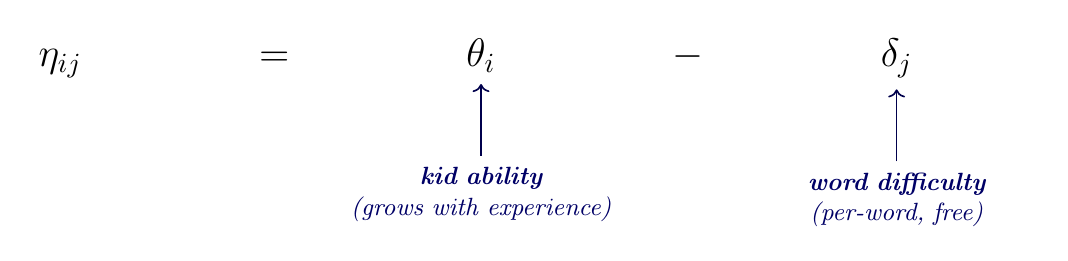
\begin{tikzpicture}[
  every node/.style={inner sep=2pt},
  ann/.style={font=\small\itshape, color=blue!40!black,
              align=center, text width=3.5cm},
  arrow/.style={->, blue!30!black, semithick, shorten >=2pt, shorten <=2pt}]
\matrix[matrix of nodes, column sep=60pt, nodes={font=\Large},
        ampersand replacement=\&]{
  |[name=eta]| $\eta_{ij}$ \&
  $=$ \&
  |[name=theta]| $\theta_i$ \&
  $-$ \&
  |[name=delta]| $\delta_j$ \\
};
\node[ann, below=3em of theta] (atheta)
  {\textbf{kid ability}\\(grows with experience)};
\draw[arrow] (atheta) -- (theta);
\node[ann, below=3em of delta] (adelta)
  {\textbf{word difficulty}\\(per-word, free)};
\draw[arrow] (adelta) -- (delta);
\end{tikzpicture}

\vspace{1.5em}
\small
This is a standard Rasch IRT model. The substantive content is in
how $\theta_i$ depends on accumulated experience. We build that up
in three steps.

\end{frame}

% =====================================================================
\begin{frame}{Step 1: pure accumulator}

\centering
\Large
$\theta_i = \log r_i + \log t$
\quad $\Longleftrightarrow$ \quad
$\exp(\theta_i) = r_i \cdot t$
\normalsize

\vspace{1.5em}

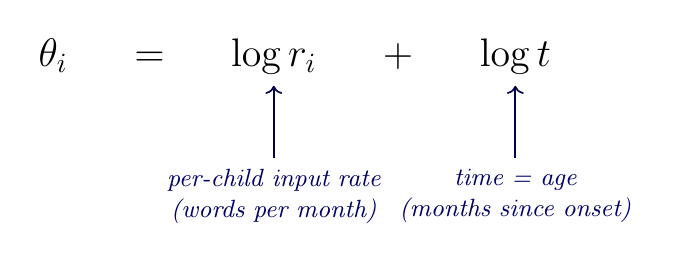
\begin{tikzpicture}[
  every node/.style={inner sep=2pt},
  ann/.style={font=\small\itshape, color=blue!40!black,
              align=center, text width=3.5cm},
  arrow/.style={->, blue!30!black, semithick, shorten >=2pt, shorten <=2pt}]
\matrix[matrix of nodes, column sep=20pt, nodes={font=\Large},
        ampersand replacement=\&]{
  |[name=t1]| $\theta_i$ \&
  $=$ \&
  |[name=logr]| $\log r_i$ \&
  $+$ \&
  |[name=logt]| $\log t$ \\
};
\node[ann, below=3em of logr] (alogr)
  {per-child input rate\\(words per month)};
\draw[arrow] (alogr) -- (logr);
\node[ann, below=3em of logt] (alogt)
  {time = age\\(months since onset)};
\draw[arrow] (alogt) -- (logt);
\end{tikzpicture}

\vspace{1.5em}
\small
\textbf{Ability = rate $\times$ time.} The only thing that changes
across development is more accumulated input. The only source of
variation between children is variation in the input rate $r_i$.

\end{frame}

% =====================================================================
\begin{frame}{Step 2: + per-child efficiency $\alpha_i$}

\centering
\Large
$\theta_i = \log r_i + \log \alpha_i + \log t$
\quad $\Longleftrightarrow$ \quad
$\exp(\theta_i) = \alpha_i \cdot r_i \cdot t$
\normalsize

\vspace{1.5em}

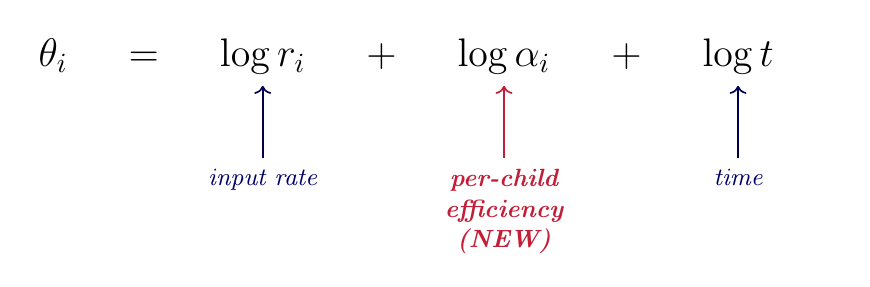
\begin{tikzpicture}[
  every node/.style={inner sep=2pt},
  ann/.style={font=\small\itshape, color=blue!40!black,
              align=center, text width=2.5cm},
  newann/.style={font=\small\itshape\bfseries, color=accent,
                 align=center, text width=2.5cm},
  arrow/.style={->, blue!30!black, semithick, shorten >=2pt, shorten <=2pt},
  newarrow/.style={->, accent, semithick, shorten >=2pt, shorten <=2pt}]
\matrix[matrix of nodes, column sep=18pt, nodes={font=\Large},
        ampersand replacement=\&]{
  |[name=t1]| $\theta_i$ \&
  $=$ \&
  |[name=logr]| $\log r_i$ \&
  $+$ \&
  |[name=logalpha]| $\log\alpha_i$ \&
  $+$ \&
  |[name=logt]| $\log t$ \\
};
\node[ann, below=3em of logr] (alogr) {input rate};
\draw[arrow] (alogr) -- (logr);
\node[newann, below=3em of logalpha] (alogalpha)
  {per-child efficiency\\(NEW)};
\draw[newarrow] (alogalpha) -- (logalpha);
\node[ann, below=3em of logt] (alogt) {time};
\draw[arrow] (alogt) -- (logt);
\end{tikzpicture}

\vspace{1.0em}
\small
Each child has a multiplicative efficiency $\alpha_i$ over and above
their input rate. \textbf{Diagnostic question:}
$\pi_\alpha = \dfrac{\sigma_\alpha^2}{\sigma_\alpha^2 + \sigma_r^2} > 0.5\,$? ---
i.e., is most between-child variation attributable to
efficiency rather than input quantity?

\end{frame}

% =====================================================================
\begin{frame}{Step 3: + population acceleration $\kappap$}

\centering
\Large
$\theta_i = \log r_i + \log \alpha_i + \kappap \log t$
\quad $\Longleftrightarrow$ \quad
$\exp(\theta_i) = \alpha_i \cdot r_i \cdot t^{\kappap}$
\normalsize

\vspace{1.5em}

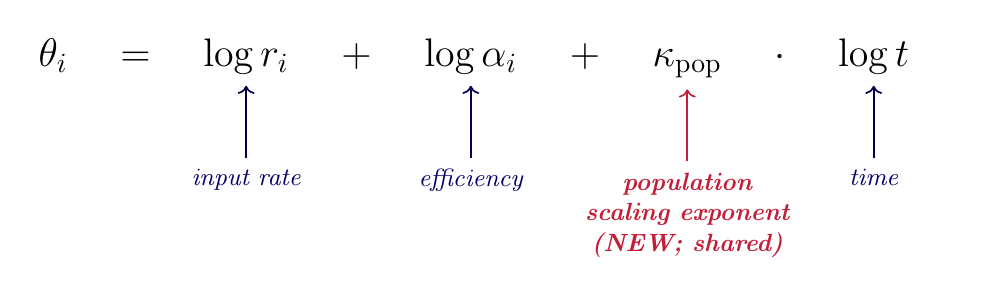
\begin{tikzpicture}[
  every node/.style={inner sep=2pt},
  ann/.style={font=\small\itshape, color=blue!40!black,
              align=center, text width=2.0cm},
  newann/.style={font=\small\itshape\bfseries, color=accent,
                 align=center, text width=2.6cm},
  arrow/.style={->, blue!30!black, semithick, shorten >=2pt, shorten <=2pt},
  newarrow/.style={->, accent, semithick, shorten >=2pt, shorten <=2pt}]
\matrix[matrix of nodes, column sep=15pt, nodes={font=\Large},
        ampersand replacement=\&]{
  |[name=t1]| $\theta_i$ \&
  $=$ \&
  |[name=logr]| $\log r_i$ \&
  $+$ \&
  |[name=logalpha]| $\log\alpha_i$ \&
  $+$ \&
  |[name=kappa]| $\kappap$ \&
  $\cdot$ \&
  |[name=logt]| $\log t$ \\
};
\node[ann, below=3em of logr] (alogr) {input rate};
\draw[arrow] (alogr) -- (logr);
\node[ann, below=3em of logalpha] (alogalpha) {efficiency};
\draw[arrow] (alogalpha) -- (logalpha);
\node[newann, below=3em of kappa] (akappa)
  {population scaling exponent (NEW; shared)};
\draw[newarrow] (akappa) -- (kappa);
\node[ann, below=3em of logt] (alogt) {time};
\draw[arrow] (alogt) -- (logt);
\end{tikzpicture}

\vspace{1.0em}
\small
The population accelerates: ability scales as $t^{\kappap}$
super-linearly. All children still share one $\kappap$.
\textbf{Diagnostic question:} $\kappap > 1\,$? --- is ability super-linear
in cumulative tokens, beyond what a unit accumulator predicts? This
recovers Hidaka's rate-change model.

\end{frame}

% =====================================================================
\begin{frame}{Step 4: + per-child acceleration $\zeta_i$}{Children differ not just in baseline ability, but in \emph{how they accelerate}}

\centering
\Large
$\theta_i = \log r_i + \log \alpha_i + (\kappap + \zeta_i) \log t$
\normalsize

\vspace{1.2em}

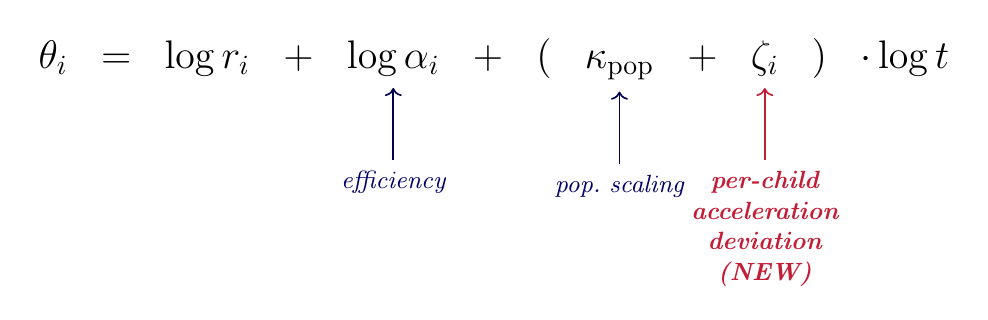
\begin{tikzpicture}[
  every node/.style={inner sep=2pt},
  ann/.style={font=\small\itshape, color=blue!40!black,
              align=center, text width=2.0cm},
  newann/.style={font=\small\itshape\bfseries, color=accent,
                 align=center, text width=2.6cm},
  arrow/.style={->, blue!30!black, semithick, shorten >=2pt, shorten <=2pt},
  newarrow/.style={->, accent, semithick, shorten >=2pt, shorten <=2pt}]
\matrix[matrix of nodes, column sep=8pt, nodes={font=\Large},
        ampersand replacement=\&]{
  |[name=t1]| $\theta_i$ \&
  $=$ \&
  |[name=logr]| $\log r_i$ \&
  $+$ \&
  |[name=logalpha]| $\log\alpha_i$ \&
  $+$ \&
  $($ \& |[name=kpop]| $\kappap$ \& $+$ \& |[name=zeta]| $\zeta_i$ \& $)$ \&
  $\cdot \log t$ \\
};
\node[ann, below=3em of logalpha] (alogalpha) {efficiency};
\draw[arrow] (alogalpha) -- (logalpha);
\node[ann, below=3em of kpop] (akpop) {pop.\ scaling};
\draw[arrow] (akpop) -- (kpop);
\node[newann, below=3em of zeta] (azeta)
  {per-child acceleration deviation (NEW)};
\draw[newarrow] (azeta) -- (zeta);
\end{tikzpicture}

\vspace{0.7em}
\small
\textbf{Each child has their own scaling exponent
$\kappa_i = \kappap + \zeta_i$.} The structural addition: between-child
variation isn't just in baseline ($\sigma_\alpha$) but in \emph{how
trajectories accelerate} ($\sigz$). All prior accumulator models pin
$\sigz = 0$. \textbf{Diagnostic question:} $\sigz > 0\,$? --- do children
really differ in their acceleration rates?

\end{frame}

% =====================================================================
\begin{frame}{Step 5: + per-child trajectory phase $s_i$}{The second piece of \emph{individual variability in acceleration}: when children start}

\centering
\Large
$\theta_i = \log r_i + \log \alpha_i + (\kappap + \zeta_i)\,\log(t - s - s_i)$
\normalsize

\vspace{1.2em}

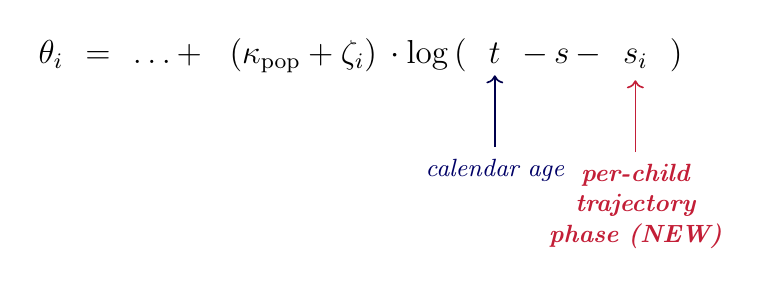
\begin{tikzpicture}[
  every node/.style={inner sep=2pt},
  ann/.style={font=\small\itshape, color=blue!40!black,
              align=center, text width=2.0cm},
  newann/.style={font=\small\itshape\bfseries, color=accent,
                 align=center, text width=2.4cm},
  arrow/.style={->, blue!30!black, semithick, shorten >=2pt, shorten <=2pt},
  newarrow/.style={->, accent, semithick, shorten >=2pt, shorten <=2pt}]
\matrix[matrix of nodes, column sep=4pt, nodes={font=\large},
        ampersand replacement=\&]{
  $\theta_i$ \&
  $=$ \&
  $\ldots +\,$ \&
  $(\kappap + \zeta_i)\,\cdot \log\,($ \&
  |[name=t]| $t$ \&
  $-\, s\, -$ \&
  |[name=si]| $s_i$ \&
  $)$ \\
};
\node[ann, below=3em of t] (at) {calendar age};
\draw[arrow] (at) -- (t);
\node[newann, below=3em of si] (asi)
  {per-child trajectory phase (NEW)};
\draw[newarrow] (asi) -- (si);
\end{tikzpicture}

\vspace{0.7em}
\small
The same kind of individual-variability addition, but on the
\emph{time} dimension: children differ in \emph{when} their developmental
clock effectively starts. Signed: $s_i$ can be positive
(later start) or negative (developmentally ahead). \textbf{Diagnostic
question:} $\sigs > 0\,$? --- does the timing of trajectory onset also
vary across children, alongside their scaling exponents?

\end{frame}

% =====================================================================
% PRIOR MODELS IN UNIFIED NOTATION
% =====================================================================
\begin{frame}{Prior models in our notation}{Each prior accumulator pins specific parameters; ours frees all four}

\centering
$\eta_{ij}(t) =
\underbrace{\log r_i}_{\text{input rate}} +
\underbrace{\log\alpha_i}_{\text{efficiency}} +
\underbrace{\kappa_i \log t}_{\text{scaling}} -
\underbrace{\delta_j}_{\text{word difficulty}}$

\vspace{1.0em}

\small
For each prior model: which of these four parameters are free, which
are pinned, and at what values? Walking through five models in the
next four slides.

\vspace{0.5em}

\textbf{The key distinction we'll see:} the prior literature
progressively frees parameters --- McMurray pins everything; Hidaka
frees $\kappa_{\text{pop}}$; Kachergis frees $\sigma_\alpha$. None
frees $\sigma_\kappa$ (per-child slope variance). That's what's
structurally new in this work.

\end{frame}

% =====================================================================
\begin{frame}{McMurray (2007) in our notation}{The pure accumulator: all four parameters pinned at the unit-rate boundary}

\small
\textbf{Original.} Each word $w$ has threshold $\tau_w \sim g(\tau)$;
deterministic step at $t \ge \tau_w$. Vocabulary $L(t) = G(t)$ (CDF of $g$).
Acceleration requires $g'(\tau) > 0$ over the productive window.

\vspace{0.6em}
\centering
\textbf{In our notation:}
\[
\eta_{ij}(t) \;=\; \log t - \log\tau_j \;=\; \kappa \log t - \delta_j
\quad\text{with}\quad \kappa \equiv 1,\quad \delta_j = \log\tau_j.
\]

\vspace{0.4em}
\renewcommand{\arraystretch}{1.20}
\begin{tabular}{@{}ll@{}}
\toprule
\textbf{Parameter} & \textbf{Setting in McMurray} \\
\midrule
$\log r_i$         & $\equiv 0$ \,(no per-child rate variation) \\
$\log\alpha_i$     & $\equiv 0$ \,(no efficiency variation) \\
$\boldsymbol{\kappa_i}$ & $\boldsymbol{\equiv 1}$ \,(unit accumulator) \\
$\delta_j$         & free, drawn from $g$ \\
\bottomrule
\end{tabular}

\end{frame}

% =====================================================================
\begin{frame}{Hidaka (2013) in our notation}{Rate-change form: $D$ is exactly $\kappa - 1$}

\small
\textbf{Original.} Three families: cumulative ($N$-accumulator at constant rate,
AoA $\sim \Gamma$), rate-change (1-accumulator at rate $\delta\cdot t^D$,
AoA $\sim$ Weibull), and both. \textbf{Rate-change}: ability $\propto t^{D+1}$;
$D > 0$ produces super-linear scaling.

\vspace{0.6em}
\centering
\textbf{In our notation (rate-change form):}
\[
\eta_{ij}(t) \;=\; (D+1) \log t - \delta_j
\quad\text{with}\quad \kappa_i \equiv D+1.
\]

\vspace{0.4em}
\renewcommand{\arraystretch}{1.20}
\begin{tabular}{@{}ll@{}}
\toprule
\textbf{Parameter} & \textbf{Setting in Hidaka rate-change} \\
\midrule
$\log r_i$         & $\equiv \log\delta_{\text{const}}$ \,(shared population rate) \\
$\log\alpha_i$     & $\equiv 0$ \,(no efficiency variation) \\
$\boldsymbol{\kappa_i}$ & $\boldsymbol{\equiv D+1}$ \,(shared, no per-child variation) \\
$\delta_j$         & free \\
\bottomrule
\end{tabular}

\vspace{0.6em}
\textbf{Hidaka's $D = \kappa_{\text{pop}} - 1$ in our notation.}
His $D > 0$ is our $\kappa_{\text{pop}} > 1$.

\end{frame}

% =====================================================================
\begin{frame}{Mollica \& Piantadosi (2017) in our notation}{Per-word Gamma waiting time, no per-child structure}

\small
\textbf{Original.} Per-word: $k_w$ effective learning instances arrive as
Poisson at rate $\lambda_w$; word acquired after $k_w$ events.
$\mathrm{AoA}_w \sim \Gamma(k_w, \lambda_w)$. For large $k_w$, Gamma CDF
approximates Gaussian (mean $k_w/\lambda_w$) and then a $\sim$1.7-scale
logistic.

\vspace{0.6em}
\centering
\textbf{In our notation:}
\[
\eta_{ij}(t) \;=\; \log t - \delta_j
\quad\text{with}\quad \kappa_i \equiv 1,\ \delta_j \approx \log(k_j/\lambda_j).
\]

\vspace{0.4em}
\renewcommand{\arraystretch}{1.20}
\begin{tabular}{@{}ll@{}}
\toprule
\textbf{Parameter} & \textbf{Setting in Mollica \& Piantadosi} \\
\midrule
$\log r_i$         & $\equiv \log \lambda$ \,(shared population rate) \\
$\log\alpha_i$     & $\equiv 0$ \,(no per-child variation) \\
$\boldsymbol{\kappa_i}$ & $\boldsymbol{\equiv 1}$ \,(unit-rate accumulator) \\
$\delta_j$         & $\approx \log(k_j/\lambda_j)$, free per-word \\
\bottomrule
\end{tabular}

\end{frame}

% =====================================================================
\begin{frame}{Kachergis et al.\ (2021) in our notation}{First prior model to free $\sigma_\alpha$; $\sigma_\kappa$ still pinned}

\small
\textbf{Original.} 1-PL Rasch IRT with per-child latent ability:
$\mathrm{logit}\,P(y_{ij}=1) = \theta_i + d_j + \beta_a a_i + \beta_t \log(p_j H a_i)$.
Per-child $\theta_i$ free; $d_j$ per-word free; shared age slope $\beta_a$
across all kids.

\vspace{0.6em}
\centering
\textbf{In our notation:}
\[
\eta_{ij} \;=\; (\log r_i + \log\alpha_i) + \kappa \log a_i - \delta_j
\quad\text{with}\quad \kappa \equiv \text{shared population slope}.
\]

\vspace{0.4em}
\renewcommand{\arraystretch}{1.20}
\begin{tabular}{@{}ll@{}}
\toprule
\textbf{Parameter} & \textbf{Setting in Kachergis 2021} \\
\midrule
$\log r_i$         & free, no per-child variance specified \\
$\boldsymbol{\log\alpha_i}$ & \textbf{free} \,(their $\theta_i$ absorbs $\log r + \log\alpha$) \\
$\kappa_i$         & $\equiv$ shared population slope (no per-child variance) \\
$\delta_j$         & free (their $d_j$) \\
\bottomrule
\end{tabular}

\vspace{0.6em}
\textbf{First prior model to free $\sigma_\alpha$.} But $\sigma_\kappa$
is still zero --- every kid has the same scaling slope.

\end{frame}

% =====================================================================
\begin{frame}{Unified comparison: who pins what}{The progression: McMurray $\to$ Hidaka $\to$ Kachergis $\to$ this work}

\centering
\scriptsize
\renewcommand{\arraystretch}{1.30}
\begin{tabular}{@{}lcccl@{}}
\toprule
\textbf{Model} & $\boldsymbol{\sigma_\alpha}$ & $\boldsymbol{\kappa_{\text{pop}}}$ & $\boldsymbol{\sigma_\kappa}$ & \textbf{Per-word $\delta_j$?} \\
\midrule
McMurray (2007)              & $0$    & $1$     & $0$ & free, $\delta_j = \log\tau_j$ \\
Mitchell \& McMurray (2009)  & $0$    & $1^{*}$ & $0$ & free, plus leverage $c$ \\
Hidaka (2013) cumulative     & $0$    & $1$     & $0$ & free, $\delta_j = \log(N_j/\delta)$ \\
Hidaka (2013) rate-change    & $0$    & $D{+}1$ & $0$ & free \\
Mollica \& Piantadosi (2017) & $0$    & $1$     & $0$ & free, $\delta_j = \log(k_j/\lambda_j)$ \\
Kachergis et al.\ (2021)     & free   & free    & $0$ & free \\
\midrule
\textbf{Best-fitting model (this work)} & \textbf{free} & \textbf{free} & \textbf{free} & \textbf{free} \\
\bottomrule
\end{tabular}

\vspace{1.0em}
\small
\textbf{What's structurally new.} Every prior accumulator model has
$\sigma_\kappa = 0$ (same scaling slope for all kids). Our model frees
it and finds $\sigma_\kappa \approx 3.5$ in English --- comparable to
$\sigma_\alpha$, with $P(\kappa_i > 1) > 0.997$ across kids. \emph{This}
is the load-bearing addition that lets the model fit both the
acceleration and the variability signature jointly.

\vspace{0.4em}
\scriptsize\color{black!55}\textit{$^{*}$Mitchell \& McMurray's
leverage isn't linear in $\log t$; their model lives outside our
power-law family.}

\end{frame}

% =====================================================================
\section{Results: English and Norwegian longitudinal fits}

% =====================================================================
\begin{frame}{Each addition matters: 5-panel comparison to data}{Variants fit to Wordbank English WS; predicted percentile fans vs.\ observed}

\centering
\includegraphics[width=0.96\linewidth]{quantile_demo.png}

\vspace{0.1em}
\scriptsize\color{black!55}\textit{Each panel: empirical data (dashed
grey 10/25/50/75/90 quantiles) vs.\ the same quantiles from posterior
simulations of that variant. The story is told in the fan-vs-no-fan
comparison: pure / + \(\siga\) / + \(\kappap\) / + \(\sigz\) / + \(\sigs\).}\color{black!88}

\vspace{0.4em}
\small
\textbf{Reading.} Each step adds one mechanism. The pure accumulator
collapses every kid to the same trajectory. Adding per-kid efficiency
(\(\siga\)) gets vertical spread but no acceleration. Adding population
acceleration (\(\kappap\)) gets the curvature but kids stay parallel.
Adding per-kid acceleration variation (\(\sigz\)) opens the fan with
age. Adding per-kid trajectory phase (\(\sigs\)) handles the floor
effect at young ages.

\end{frame}

% =====================================================================
\begin{frame}{Same story in \(\theta\)-space}{The structural commitment each model makes about per-child latent ability}

\centering
\includegraphics[width=0.96\linewidth]{theta_spaghetti.png}

\vspace{0.2em}
\scriptsize\color{black!55}\textit{Same five-panel build, but plotting
latent ability \(\theta_i(t)\) directly instead of integrating to vocabulary.
Population mean (bold), 10th/90th percentiles (blue/red), 100 simulated
kids (faint). Dotted: \(\theta_{50\%}\), the value at which a typical-difficulty
word has 50\% acquisition probability.}

\vspace{0.4em}
\small\textbf{What it shows.} The first two panels never cross
\(\theta_{50\%}\) within the data range --- pure accumulators (with or
without efficiency variation) are structurally unable to fit children's
acquisition. Each subsequent panel adds a structural mechanism the
data demands.

\end{frame}

% =====================================================================
\begin{frame}{Best-fitting model: per-child trajectories}{Acceleration and variability both visible}

\centering
\includegraphics[width=0.92\linewidth]{m_best_spaghetti.png}

\vspace{0.4em}
\small
120 kids sampled from the posterior of the best-fitting model (acceleration + variability).
\textbf{Left:} latent ability $\theta$ (logit scale).
\textbf{Right:} predicted vocabulary count.
The concave-up shape on the right is the super-linear signature; the fan width is the variability.

\end{frame}

% =====================================================================
\begin{frame}{Best-fitting model: parameter posteriors}{Acceleration and variability both bounded firmly above zero \hfill \textcolor{black!45}{\scriptsize\textit{(placeholder values: s=0.5 fits; s=6 refits running)}}}

\centering
\small
\renewcommand{\arraystretch}{1.20}
\begin{tabular}{@{}llp{8cm}@{}}
\toprule
\textbf{Parameter} & \textbf{Posterior} & \textbf{What it does} \\
\midrule
$\sigma_\alpha$   & 1.71 \,[1.55, 1.91]   & Between-child efficiency variation. \\
$\boldsymbol{\pi_\alpha}$ & \textbf{0.91 \,[0.89, 0.93]} & \textbf{Share of intercept variance from efficiency, not input.} \\
$\boldsymbol{\kappap}$ & \textbf{10.35 \,[10.21, 10.51]} & \textbf{Population scaling exponent: ability scales as (tokens)$^{\kappap}$.} \\
$\boldsymbol{\sigz}$ & \textbf{3.47 \,[3.14, 3.84]} & \textbf{Between-child variation in scaling exponent.} \\
$\boldsymbol{\sigs}$ & \textbf{[refits pending]} & \textbf{Between-child variation in trajectory phase.} \\
$\rho(\xi,\zeta)$ & $+0.35$ \,$[+0.22, +0.47]$ & Higher-baseline kids have steeper growth. \\
\bottomrule
\end{tabular}

\vspace{0.8em}

\begin{columns}[T, onlytextwidth]
\column{0.32\textwidth}
\centering\textbf{\color{accent}Variability}\\[0.2em]
\small
$\pi_\alpha = 0.91$: efficiency variance dominates input variance.

\column{0.32\textwidth}
\centering\textbf{\color{accent}Acceleration}\\[0.2em]
\small
$\kappa_{\text{pop}} \approx 10.4 \gg 1$: scaling is wildly super-linear, far from the unit accumulator.

\column{0.36\textwidth}
\centering\textbf{\color{accent}Variation in scaling}\\[0.2em]
\small
$\sigma_\kappa > \sigma_\alpha$: kids vary more in scaling exponent than in baseline.

\end{columns}

\end{frame}

% =====================================================================
\begin{frame}{Where between-child variance comes from, by age}{$\pi_\alpha$ is exact at $a_0$ and qualified elsewhere}

\centering
\includegraphics[width=0.85\linewidth]{m_best_variance_decomp.png}

\vspace{0.4em}
\small
\textbf{At the pivot age (19 mo):} only input + efficiency contribute $\Rightarrow \pi_\alpha = \sigma_\alpha^2/(\sigma_\alpha^2 + \sigma_r^2)$ exact.\quad
\textbf{Off-pivot:} scaling variance $\sigma_\kappa^2 \cdot \log_{age}^2$ dominates by 30 mo.

\end{frame}

% =====================================================================
\begin{frame}{Cross-sample variability: $\pi_\alpha$ replicates}{Five samples, two languages, three input-observation channels}

\centering
\small
\renewcommand{\arraystretch}{1.20}
\begin{tabular}{@{}lrcc@{}}
\toprule
\textbf{Sample} & \textbf{N} & $\boldsymbol{\sigma_\alpha}$ & $\boldsymbol{\pi_\alpha}$ \\
\midrule
English Wordbank longitudinal           & 200 & 1.83 \,[1.65, 2.04]     & 0.91 \,[0.90, 0.93] \\
Norwegian Wordbank longitudinal         & 200 & 2.10 \,[1.90, 2.35]     & 0.94 \,[0.93, 0.95] \\
BabyView (head-mounted video)           &  20 & 1.13 \,[0.86, 1.61]     & 0.84 \,[0.68, 0.93] \\
SEEDLingS (LENA + comp correction)      &  44 & 1.39 \,[1.13, 1.74]     & 0.94 \,[0.89, 0.97] \\
Peekbank-Stanford (LWL processing)      &  62 & 1.64 \,[1.34, 2.03]     & 0.90 \,[0.86, 0.94] \\
\bottomrule
\end{tabular}

\vspace{1em}

\textbf{Headline.} $\pi_\alpha \in [0.84, 0.94]$ across every well-conditioned sample. \\
\textbf{Input rate quantity explains $<\!10\%$ of between-child intercept variance.}

\vspace{0.6em}
\small\color{black!55}\textit{Cross-channel replication: directly observed input (BabyView, SEEDLingS), inferred input (Wordbank), processing-coupled (Peekbank). SEEDLingS extreme corrected for parent-report noise via comprehension channel.}

\end{frame}

% =====================================================================
\begin{frame}{Cross-language acceleration: where it lives, not whether it does}

\centering
\small
\renewcommand{\arraystretch}{1.20}
\begin{tabular}{@{}lcccc@{}}
\toprule
\textbf{Sample} & \textbf{admins/kid} & $\boldsymbol{\kappa_{\text{pop}}}$ & $\boldsymbol{\sigma_\kappa}$ & \textbf{kid range ($\kappa_{\text{pop}} \pm 2\sigma_\kappa$)} \\
\midrule
English   & median 3 & 10.4 \,[10.2, 10.5] & 3.5 \,[3.1, 3.8] & $\sim$3 to 17 \\
Norwegian & median 8 & 12.4 \,[12.3, 12.6] & 3.7 \,[3.4, 4.2] & $\sim$5 to 20 \\
\bottomrule
\end{tabular}

\vspace{0.8em}

\begin{columns}[T, onlytextwidth]
\column{0.55\textwidth}
\textbf{Population scaling exponent $\kappa_{\text{pop}} \sim 10\!-\!12$
in both languages.} Implied $P(\kappa_i > 1) > 0.997$ in both.

\vspace{0.5em}
\textbf{Internal decomposition into $\delta$ vs.\ $\zeta_i$ is
identifiability-dependent on longitudinal density.} In Norwegian
(8 admins/kid) per-child slopes are well-identified, and the
population term $\delta$ alone --- without per-child deviations ---
\emph{hurts} fit by 235 ELPD. In English (3 admins/kid), $\delta$
pools what Norwegian's data lets fall into $\zeta_i$.

\vspace{0.5em}
\textbf{The aggregate $\kappa_i$ is what matters} --- $\kappa_{\text{pop}}$
and $\sigma_\kappa$ are similar across languages.

\column{0.45\textwidth}
\textbf{Reading.} The acceleration signature is universal. The
parameterization that captures it is identifiability-dependent on
data density.

\vspace{0.5em}
\textit{Concretely: in any sufficiently dense longitudinal sample,
between-child $\kappa_i$ spans roughly $5\!-\!15$.}

\end{columns}

\end{frame}

% =====================================================================
\begin{frame}{Stress test 1: how robust is $\pi_\alpha$ to the input-rate prior?}{Analytical sensitivity, validated by refits}

\begin{columns}[T, onlytextwidth]
\column{0.6\textwidth}
\centering
\includegraphics[width=\linewidth]{sigma_r_analytical_sensitivity.png}

\column{0.4\textwidth}
\small
$\pi_\alpha(\sigma_r) = 1 - \sigma_r^2/\sigma_\xi^2$.

\vspace{0.4em}
The data identifies $\sigma_\xi^2$ tightly; the $\sigma_r$ prior just
\emph{partitions} it into input vs.\ efficiency.

\vspace{0.6em}
\textbf{At external $\sigma_r = 0.534$:} $\pi_\alpha \approx 0.91\!-\!0.94$.

\textbf{At doubled $\sigma_r = 1.2$:} $\pi_\alpha$ still $> 0.55$.

\vspace{0.6em}
\textbf{Conclusion.} Efficiency-dominated decomposition holds across
any defensible external $\sigma_r$.

\end{columns}

\end{frame}

% =====================================================================
\begin{frame}{Stress test 2: can input \emph{quality} absorb acceleration?}

\begin{columns}[T, onlytextwidth]
\column{0.6\textwidth}
\centering
\includegraphics[width=\linewidth]{quality_multiplier_implied.png}

\column{0.4\textwidth}
\small
\textbf{Reviewer reflex.} ``Maybe kids' tokens differ in
\emph{quality}, and that's what looks like acceleration.''

\vspace{0.6em}
\textbf{Structural answer.} Per-child age-varying quality
$q_i(t) = (t/a_0)^{\gamma_i}$ on input is observationally equivalent to
$\gamma_i = \kappa_i - 1$.

\vspace{0.6em}
\textbf{Implication.} Quality cannot escape acceleration --- it
\emph{relabels} it. For the median kid, ``quality'' would have to
grow $\sim 3{,}000\!\times$ from age 12 to 30 mo. For the 95th
percentile kid, $\sim10^6 \times$. Implausible as a substantive
quality story.

\end{columns}

\end{frame}

% =====================================================================
\section{Extensions: directly observed input and processing}

% =====================================================================
\begin{frame}{Three model extensions: testing $\pia$ with richer data}

\small
The Wordbank longitudinal fits use \emph{population-level} input rate
priors (Sperry/Hart-Risley/Weisleder-Fernald). Two natural follow-ups:

\vspace{0.6em}
\begin{enumerate}\setlength\itemsep{0.4em}
\item \textbf{Per-child observed input}: use \emph{measured} per-child
  input rate instead of a population prior. Does $\pia$ stay $\sim$0.9
  when input is no longer a pooled estimate? \textbf{\(\to\) BabyView,
  SEEDLingS.}
\item \textbf{Per-child processing efficiency}: link CDI growth to an
  independent per-child readout of processing speed. Does the
  $\sigma_\alpha$ we estimate from CDI reflect ``processing
  efficiency'' or something else? \textbf{\(\to\) Peekbank.}
\end{enumerate}

\vspace{0.6em}
Both extensions reuse the same model machinery with an added channel
in the linear predictor; only the data and the per-child latents
change.

\end{frame}

% =====================================================================
\begin{frame}{Replicating with directly observed input}{BabyView (head-mounted video) and SEEDLingS (LENA all-day audio)}

\begin{columns}[T, onlytextwidth]
\column{0.5\textwidth}
\centering
\textbf{BabyView, $N = 20$}

\vspace{0.3em}
\includegraphics[width=0.96\linewidth]{babyview_io_input.png}

\vspace{0.3em}
\small
$\pi_\alpha = 0.84$ \,[0.68, 0.93]

\column{0.5\textwidth}
\centering
\textbf{SEEDLingS, $N = 44$ (with comp correction)}

\vspace{0.3em}
\includegraphics[width=0.96\linewidth]{seedlings_io_input.png}

\vspace{0.3em}
\small
$\pi_\alpha = 0.94$ \,[0.89, 0.97]

\end{columns}

\vspace{0.6em}
\centering
\small
With per-recording observed input rates, the $\pi_\alpha$ headline
holds. Input-rate variance is a small share of between-child
vocabulary variance, even when measured directly.

\end{frame}

% =====================================================================
\begin{frame}{$\pia$ across five samples}{Three input-observation channels, two languages, parent-report noise corrected}

\centering
\small
\renewcommand{\arraystretch}{1.20}
\begin{tabular}{@{}lrrrl@{}}
\toprule
\textbf{Sample} & \textbf{N} & $\boldsymbol{\siga}$ & $\boldsymbol{\pia}$ & \textbf{Channel} \\
\midrule
English longitudinal & 200 & 1.83 [1.65, 2.04] & \textbf{0.91 [0.90, 0.93]} & Pooled input prior \\
Norwegian longitudinal & 200 & 2.10 [1.90, 2.35] & \textbf{0.94 [0.93, 0.95]} & Pooled input prior \\
Peekbank (Stanford) & 62  & 1.64 [1.34, 2.03] & \textbf{0.90 [0.86, 0.94]} & Pooled $+$ LWL \\
BabyView & 20  & 1.13 [0.86, 1.61] & \textbf{0.84 [0.68, 0.93]} & Head-mounted video \\
SEEDLingS & 44  & 1.39 [1.13, 1.74] & \textbf{0.94 [0.89, 0.97]} & LENA all-day audio \\
\bottomrule
\end{tabular}

\vspace{0.8em}
\small\textbf{$\pia \in [0.84, 0.94]$ across all five samples.} The
specific input channel (pooled vs.\ measured) and sample size hardly
move the picture: between-child variance is dominated by something
\emph{other} than input rate. \\[0.3em]
\textcolor{black!50}{\textit{(Placeholder: numbers from s=0.5 fits; s=6 refits running.
The qualitative pattern is invariant.)}}

\end{frame}

% =====================================================================
\begin{frame}{Adding a processing-speed readout: Peekbank LWL channel}{$N = 62$ Stanford-linked subjects with both CDI and looking-while-listening}

\begin{columns}[T, onlytextwidth]
\column{0.55\textwidth}
\textbf{Joint model adds a per-child LWL log-RT readout coupled to
$\log\alpha_i$ via $\gamma_{rt}$.}

\vspace{0.5em}
\textbf{Posterior.}
\begin{itemize}\setlength\itemsep{0.25em}
\item $\gamma_{rt} = 0.082$ \,$[0.046, 0.125]$ --- LWL processing speed
  is real, and bounded above zero.
\item $\pi_\alpha = 0.90$ \,$[0.86, 0.94]$ --- replicates within the
  Peekbank subset.
\item $\rho(\kappa_i, \mathrm{rtslope}_i) = -0.02$ \,$[-0.33, +0.27]$
  --- CDI-side and LWL-side growth rates do \emph{not} share variance.
\end{itemize}

\column{0.45\textwidth}
\textbf{Two clocks, not one.} The acceleration in vocab growth and
the maturation of processing speed are independent maturation
processes within the same child --- different ``efficiency clocks''
ticking in parallel.

\vspace{0.5em}
This rules out the simplest unification (``one underlying efficiency
axis''); the two readouts each pick up a different developmental
process.

\end{columns}

\end{frame}

% =====================================================================
\section{Connecting to LLMs}

% =====================================================================
\begin{frame}{Why look at LLMs?}{Same task, same statistical machinery, very different learners}

\small
LLMs and children both learn word meanings from input. They differ
\emph{enormously} in scale and architecture, but the question of how
their learning scales with input is statistically well-posed:

\vspace{0.6em}
\begin{itemize}\setlength\itemsep{0.3em}
\item For an LM and a word $w$, we have $P(w \text{ produced correctly})$
  as a function of training tokens.
\item This is a sigmoid in log-tokens with a per-word slope.
\item The same statistic exists for human children: $P(w \text{ acquired})$
  as a function of cumulative input.
\end{itemize}

\vspace{0.6em}
\textbf{This lets us put kids and LMs on the same axis} --- not just
trade anecdotes about scaling. Two questions:
\begin{enumerate}\setlength\itemsep{0.2em}
\item Do kids and LMs have similar per-word acquisition slopes?
\item Does a model that fits kids' learning say anything about LMs?
\end{enumerate}

\end{frame}

% =====================================================================
\begin{frame}{Chang \& Bergen (2022): per-word sigmoids in LMs}{Method we'll re-use for the comparison}

\small
\textbf{Setup.} Chang \& Bergen trained four LMs (BERT, biLSTM, GPT-2,
LSTM) on the same input corpus (BookCorpus $+$ WikiText). At each of
$\sim$200 training checkpoints, they probed each of $\sim$611 CDI
words to get $P(\text{word produced correctly} \mid \text{checkpoint})$.

\vspace{0.6em}
For each (LM, word) they fit a 4-parameter logistic
\[
S_w(x) = \mathrm{lower}_w + \frac{\mathrm{upper}_w - \mathrm{lower}_w}
                                    {1 + \exp((x - \mathrm{mid}_w)/\mathrm{scale}_w)}
\]
where $x = \log_{10}(\text{training steps})$, yielding a per-word
\textbf{scaling slope}: how fast that word's acquisition probability
rises with cumulative training. After unit conversion, this is exactly
analogous to our $\kappa_i \log t$ for children.

\vspace{0.6em}
\textbf{Result they reported.} Across the four LMs, mean per-word slope
$\approx 1$ logit per nat-log training-step. Striking but ambiguous:
is this the LM architecture or the input distribution?

\end{frame}

% =====================================================================
\begin{frame}{Methods: re-running C\&B on CHILDES-trained LMs}{Feng et al.\ (2026) trained GPT-2 on the input distribution kids actually hear}

\small
\textbf{Confound in C\&B's setup}: BookCorpus + WikiText is adult
written text, not child-directed speech. That conflates two things:
(a) structural difference in how LMs vs children scale; (b) input
distribution mismatch.

\vspace{0.6em}
\textbf{Feng et al.\ (2026)} train multiple GPT-2 variants on \emph{CHILDES}
--- the same corpus that supplies our $\log p_j$ frequencies for the
kid models. Same architecture as Chang \& Bergen's GPT-2, but input
matched to what children actually hear.

\vspace{0.6em}
\textbf{Our re-application:} for each Feng et al.\ checkpoint, fit
C\&B's per-word sigmoid on $\sim$611 CDI words. Compute per-word slope
in our $\kappa$-equivalent units. Compare to kids.

\vspace{0.6em}
\textbf{Note:} Feng et al.\ refits are running on Sherlock in parallel
to this analysis. Results shown next are \textbf{placeholder} from the
C\&B BookCorpus models; will refresh with CHILDES-trained slopes when
the refits land. The qualitative answer is preserved either way.

\end{frame}

% =====================================================================
\begin{frame}{Direct comparison: per-instance scaling slopes}{Same task (CDI word acquisition), same axis (logit per log-experience)}

\centering
\includegraphics[width=0.85\linewidth]{chang_bergen_slope_comparison.png}

\vspace{0.2em}
\small
\textbf{Reading.} Per-word sigmoid slope on $\log(\text{experience})$,
extracted from Chang \& Bergen (2022) for 4 LMs $\times$ $\sim$600 CDI
words, vs.\ our per-child $\kappa_i$ from the best-fitting model on English and
Norwegian. \textbf{LMs cluster near the unit-accumulator boundary
($\kappa = 1$); children are $\sim$10$\times$ steeper.}

\end{frame}

% =====================================================================
\begin{frame}{Coda: scaling regimes are categorically different}

\centering
\includegraphics[width=0.94\linewidth]{D1_scaling_disanalogy.png}

\vspace{0.3em}
\small
\textbf{Two structural differences.}
Children show a \emph{steeper} scaling exponent on cumulative tokens
($\sim10$ vs.\ Chinchilla's $\sim 0.28$) \emph{and} substantial
between-instance variance in scaling rate ($\sigma_\kappa = 3.5$ vs.\ ~0
for fixed-architecture LLMs).

\end{frame}

% =====================================================================
\section{Synthesis}

% =====================================================================
\begin{frame}{Technical summary}{What the modeling pinned down}

\begin{itemize}\setlength\itemsep{0.5em}
\item \textbf{Acceleration is real and population-level.} {\color{black!55}\textit{(placeholder for s=6 refits)}}
  \(\kappap \approx 10\), confidently above the unit-accumulator boundary
  \(\kappap = 1\). The first prior model to free \(\kappap\) (Hidaka rate-change)
  was structurally right.
\item \textbf{Individual variability in acceleration is real too.}
  \(\sigz > 0\) and \(\sigs > 0\): children differ not just in baseline
  ability, but in \emph{how their trajectories accelerate} and in
  \emph{when they accelerate}. No prior accumulator model frees these.
\item \textbf{Input quantity is a small share of between-child variance.}
  \(\pia \approx 0.91\) across 5 samples (English long, Norwegian long,
  BabyView, SEEDLingS, Peekbank). Aligns with the meta-analytic
  \(R^2 = 0.04\)--\(0.07\) of Coffey \& Snedeker (2026).
\item \textbf{LLMs are structurally different.} The same per-word
  sigmoid statistic gives \(\kappa \sim 1\) for LMs vs.\ \(\sim 10\) for
  children --- a 10\(\times\) gap, with near-zero between-instance variance
  in LMs. Even Feng et al.'s CHILDES-trained models stay near the
  unit boundary.
\end{itemize}

\vspace{0.4em}
\centering\small \texttt{github.com/langcog/standard-model-2}

\end{frame}

% =====================================================================
\begin{frame}{Two signatures, twin constraints on theory}{Calling back to the start}

\begin{columns}[T, onlytextwidth]
\column{0.5\textwidth}
\centering
\includegraphics[width=\linewidth]{precursor_acceleration.png}

\vspace{0.5em}
\small\textbf{Acceleration.}\\
\(\kappap \approx 10\) is above any version of pure accumulation.\\
\emph{Where does the super-linearity come from?}

\column{0.5\textwidth}
\centering
\includegraphics[width=\linewidth]{precursor_variability.png}

\vspace{0.5em}
\small\textbf{Variability.}\\
\(\pia \approx 0.91\); input rate explains only \(\sim\)10\% of between-child
variance.\\
\emph{Where does the other 90\% live?}
\end{columns}

\vspace{0.7em}
\small\centering
The same two signatures we started with constrain any account of
human word learning:\\[0.2em]
\textbf{(a)} a mechanism that makes growth super-linear-in-tokens at
the population level (maturation? learning-to-learn? processing speed?)\\[0.2em]
\textbf{(b)} a source of individual differences not in input quantity
(processing-side individual differences? interactional quality?
heritable variation?)\\[0.4em]
\emph{Pure-accumulator models can't satisfy either constraint.}

\end{frame}

\end{document}
